\section{ADB (Android Debug Bridge)}
\subsection{Grundlagen}
Die Android Debug Bridge ist eine Softwaresuite mit der es möglich ist, von Host PCs mit Android Geräten zu kommunizieren.
Der Hauptnutzen besteht darin, Android Applikationen in einem virtuellen Gerät (Emulator) oder direkt auf echten Geräten zu debuggen.
Dabei wird auf dem Host ein Server gestartet, welcher die Kommunikation zwischen Host und Endgerät übernimmt. 

Die Clients (z.B. das adb command line tool, oder IDEs wie Android Studio), verbinden sich mit dem Server und senden Befehle an das über USB (oder Wifi) mit dem Server verbundene Endgerät.
Auf den Endgeräten oder im Emulator läuft im Hintergrund ein Dienst, der die Kommandos vom Server entgegennimmt und antwortet. Die Kommunikation mit dem Server läuft über TCP,
was es Clients ermöglicht sich über das Netzwerk mit Servern zu verbinden. (Siehe Abbildung \ref{adb})
\begin{figure}
	\centering
	\caption{Android Debug Bridge Architektur}
	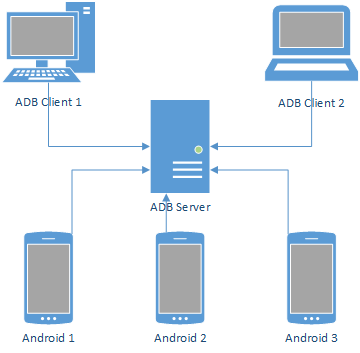
\includegraphics[width=0.4\textwidth]{media/adb.png}	
	\label{adb}
\end{figure}

Der ADB Dienst auf den Endgeräten muss explizit durch den Nutzer aktiviert werden, bevor er benutzt werden kann.
Da adb für das debuggen von Apps, also für Softwareentwickler konzipiert ist, stellt dies im allgemeinen kein Usability Problem dar. 
Das ADB Protokoll selbst ist sehr einfach gehalten, so dass eine eigenständige Reimplementierung möglich ist.
Die Kommunikation läuft dabei über einfache Message Pakete, in denen verschiedene Kommandos enthalten sein können.
\lstset{language=C,
	basicstyle=\ttfamily\scriptsize
}
\lstinputlisting{code/adb_struct_message.c}
  

\subsection{Verwendung mit externen Geräten}
Außer dem benutzten der ADB zum debuggen, kann die Architektur auch benutzt werden, um eigene Kommunikationsprotokolle zu implementieren.
Dabei wird das eigene Protokoll als eine Zusatzschicht über adb, in Form von Kommandos implementiert. TODO ??


TODO wann von wem zur Device kommunikation ?? --> IOIO

